
%%%%%%%%%%%%%%%%%%%%%%%%%%%%%%%%%%%%%%%%%%%%%%%%%%%%%%%%%%%%%
%% HEADER
%%%%%%%%%%%%%%%%%%%%%%%%%%%%%%%%%%%%%%%%%%%%%%%%%%%%%%%%%%%%%

\documentclass[a4paper, onecolumn, oneside, 11pt]{article}
\usepackage{cmbright}
\usepackage[T1]{fontenc}
\usepackage[english]{babel}

%\usepackage[dvips]{graphics} %%graphics and normal LaTeX
%\usepackage{amsmath}
%\usepackage{amsthm}
%\usepackage{amsfonts}
\usepackage{amssymb}
\usepackage{graphicx}
\usepackage{rotating}
\usepackage{pdflscape} 
\usepackage{abstract}
\usepackage[ table ]{ xcolor }
\usepackage[square, comma, sort&compress, longnamesfirst]{natbib} %
\usepackage{subfigure}
\usepackage{setspace}
%\singlespacing %% 1-spacing (default)s
%\onehalfspacing
\newcommand{\degree}{$^{\circ}$\ }
%%% END Article customizations

%%% The "real" document content comes below...

\title{Saccadic Biases}

\author{Alasdair D. F. Clarke, Matthew J. Stainer}


%\date{} % Activate to display a given date or no date (if empty),

% otherwise the current date is printed

\begin{document}

\maketitle

\begin{abstract}
More bias modelling! Cause who can be bothered running actual experiments?


Much effort has been made to attempting to explain eye guidance during natural scene viewing [Tatler, 2009 VIS RES special issue]. However, underlying fixation placement appears to be a set of consistent biases in eye movement behaviour (e.g. see Clarke and Tatler, 2014). We present a model that parametrically accounts for where saccades are directed dependent on where in the bounds of a scene an observer is currently fixating. We find... [some very interesting stuff]. Given that much of our understanding in eye guidance is derived from how people look at pictures on a computer screen, it is important that we use these biases to form a frame upon which to build more sophisticated models of eye guidance that can account for the allocation of gaze above oculomotor behaviours that are independent of the image.

\end{abstract}

%%%%%%%%%%%%%%%%%%%%%%%%%%%%%%%%%%%%%%%%%%%%%%%%%%%%%%%%%%
\section{Introduction}
%%%%%%%%%%%%%%%%%%%%%%%%%%%%%%%%%%%%%%%%%%%%%%%%%%%%%%%%%%

Improve on last year's \citep{clarke-tatler2014} effort. More sophisticated biases. And some examples of how to use biases for improved data analysis. 

The human fovea provides a small window of high acuity vision to the world, and as such the locations that we select to view in the world can tell us about how we seek the information necessary to complete the task we are currently undertaking. Current understanding of eye guidance would suggest that fixation locations are selected based on a combination of low-level factors (such as visual salience \citep{Itti:2000te} or orientation information \citep{Baddeley:2006wq}) and high-level factors \citep{Yarbus:1967wd, Buswell:1935tf, Land:2001uc}. However, there are also strong observable biases in eye movement including directional and amplitudinal [XXis that a word?XX] biases in saccades \citep{Tatler:2008uu, Tatler:2009vp, Foulsham:2010fj}, and a strong tendency to fixate near to the centre of images \citep{Tatler:2007hk,Canosa:2003tu}. Importantly, these biases are independent of the viewed content. If we are to gain a complete understanding of the factors that govern eye movement, we must therefore build models of eye guidance on the framework of these underlying biases.

\subsection{The central bias}
There is a strong tendency for people to look close to the centre of pictures \citep{Tatler:2007hk,Tatler:2005bw, Canosa:2003tu, Clarke:2014km} and movies \citep{Tseng:2009jn} presented on computer screens. There have been a number of suggestions for why this might be. One possibility for this effect is that the muscles of the eye show a preference for the `straight ahead' position, re-centring in the orbit of the eye socket for most comfortable contraction of the ocular muscles (an \emph{orbital reserve} \citep{Fuller:1996bx}). As most scene viewing experimental set-ups stabilise the head to increase the accuracy of the eye tracking, and most scenes are presented in the centre of computer displays, such a re-centring mechanism would mean that the centre of images would indeed be preferentially selected. However, when scenes are scrambled into four quadrants, fixations are located near to the centre of each quadrant, rather than the display centre, suggesting that the central tendency is responsive to the viewed content \citep{Stainer:2013ce} rather than the frames of the computer monitor.

Another possibility for the central fixation bias is that it represents a \emph{photographer bias} as photographers tend to frame their shots to include the most important content in the centre of the scene. However, when \cite{Tatler:2007hk} presented scenes where the image features were biased towards the edge of the scene, the central fixation bias persisted. The final possibility is that as a consequence of repeated exposure to photographer bias, the centre of scenes is simply where people are \emph{trained} to look at images \citep{Parkhurst:2002vo}. Such learning of spatial probabilities of targets can explain why, for example, people tend to look around the horizon when searching for people in natural scenes \citep{Birmingham:2009hl, Torralba:2006iq, Ehinger:2009ji}. Expecting to find interesting content in the centre of scenes might be a consequence of this hypothesis typically being correct.

\cite{clarke-tatler2014} revealed that the characteristics of the central bias is remarkably consistent across a series of eye movement databases.... [obviously you are in a better place than me to talk about this paper!]



\subsection{Behavioural biases in saccades}
Further to the observed bias towards the centre of images, it has been revealed that there are underlying biases in the characteristics of eye movement (in terms of the directions and amplitudes of saccades). It has been noted by several researchers that when viewing scenes, there is a higher proportion of eye movements in horizontal directions than vertical or oblique movements (Brandt, 1945; Crundall \& Underwood, 1998; Gilchrist \& Harvey, 2006; Foulsham, Kingstone \& Underwood, 2008; Tatler \& Vincent, 2008). There are a number of possibilities as to why this tendency exists (as discussed in Foulsham, Kingstone, \& Underwood, 2008). Firstly, there may be a muscular or neural dominance making oculomotor movements in the horizontal directions more likely. Secondly, the characteristics of photographic images may mean that content tends to be arranged horizontally by the photographer. In such situations, horizontal saccades may be the most efficient way to inspect scenes. Thirdly, using horizontal saccades in scene viewing might be a learned strategy. Observers may learn the natural characteristics of scenes based on previous experience, and therefore demonstrate an increased likelihood of moving in the horizontal direction. A final alternative explanation is that this tendency is a consequence of the aspect ratio of visual displays, which normally allow for larger amplitude saccades in the horizontal than vertical directions (Wartburg et al., 2007).

Foulsham and colleagues have presented two interesting exceptions to the horizontal direction bias. Foulsham, Kingstone and Underwood (2008) found that when the orientation of an image is rotated, the distribution of saccade directions follows the orientation of the scene. A second exception comes from using circular apertures (Foulsham \& Kingstone, 2010). When a scene is presented in a circular aperture, the tendency to make horizontal saccades disappears, being replaced by a tendency to make vertical saccades relative to the image orientation. However, when using fractal images (where images do not have an obvious orientation), observers tend make horizontal saccades, regardless of the angle that the image is presented.

\begin{figure}
\centering
\subfigure[]{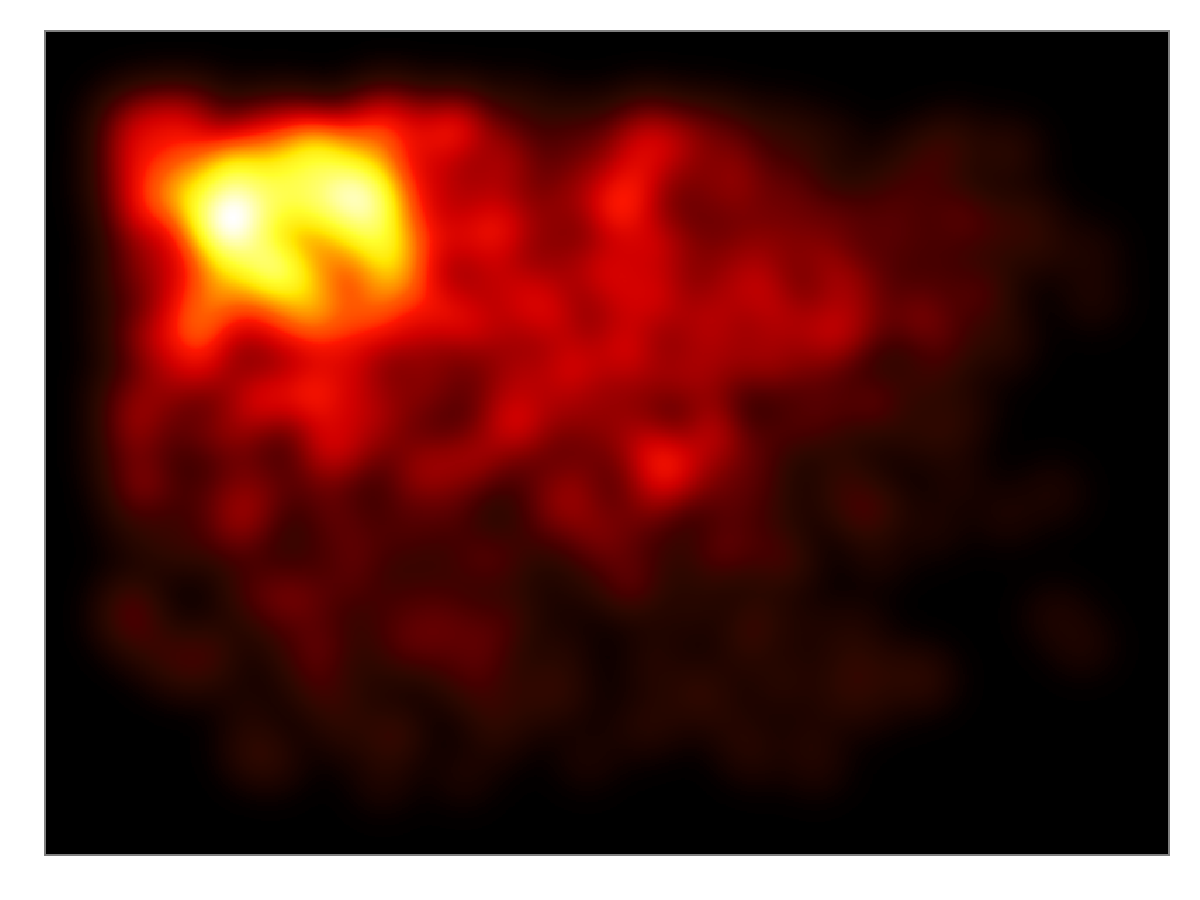
\includegraphics[width=3cm]{../scripts/heatmaps/SaccadicFlowMaps/Figures/BBias_11.pdf}}
\subfigure[]{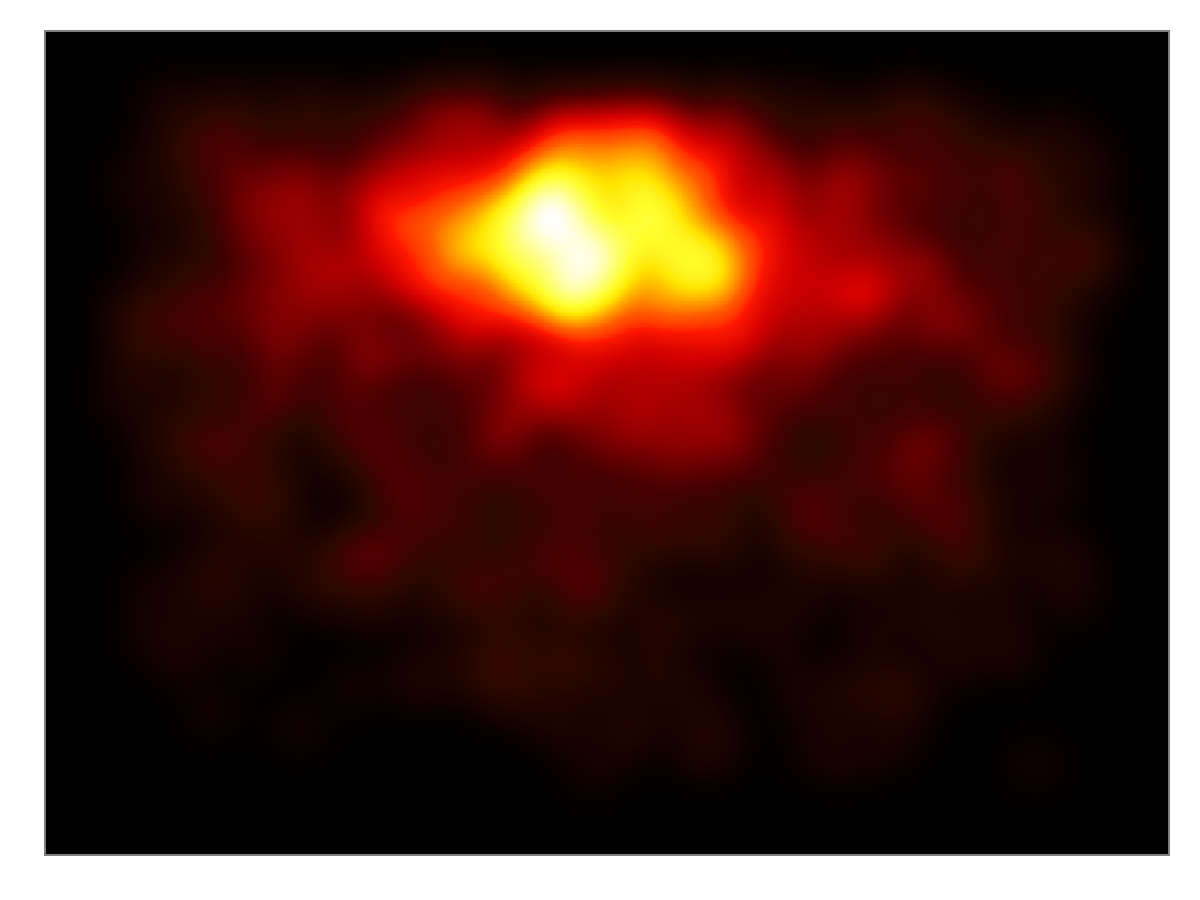
\includegraphics[width=3cm]{../scripts/heatmaps/SaccadicFlowMaps/Figures/BBias_12.pdf}}
\subfigure[]{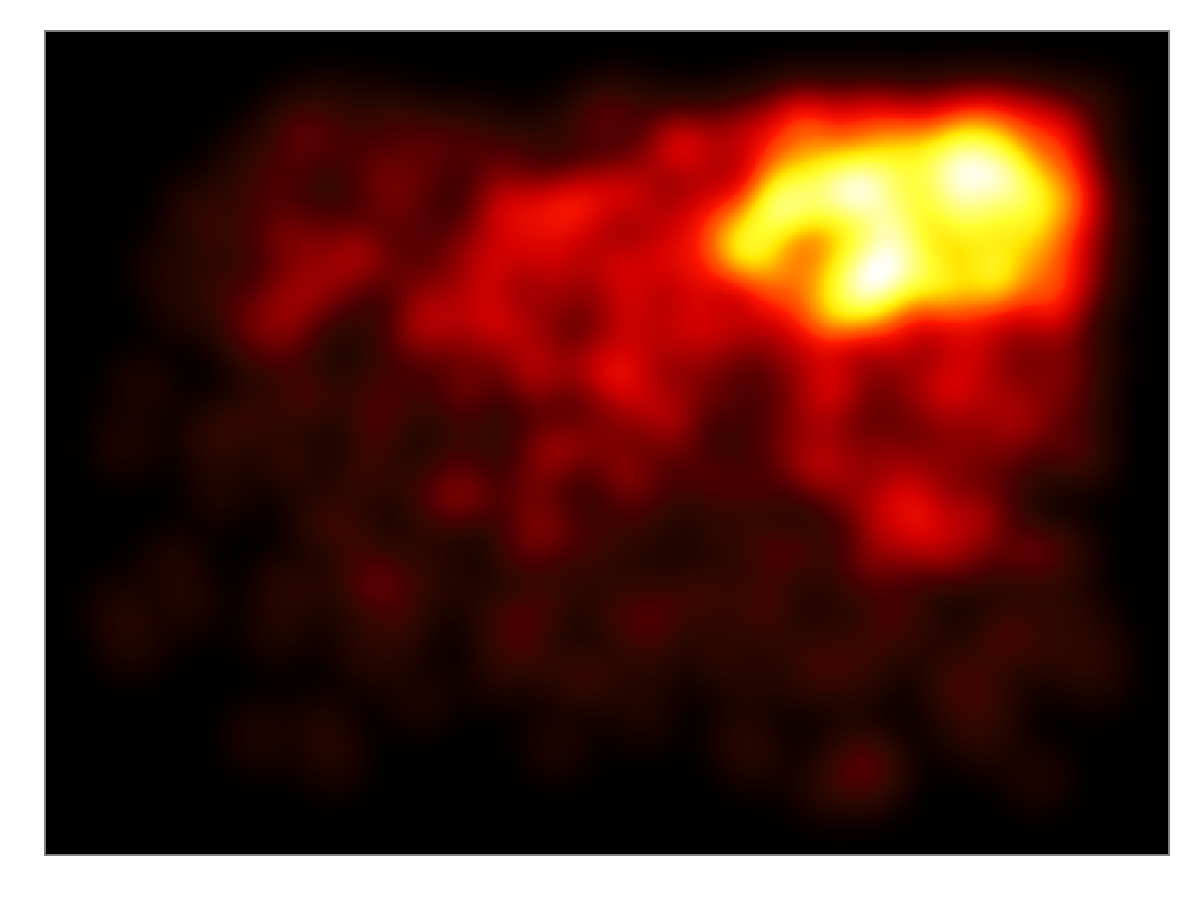
\includegraphics[width=3cm]{../scripts/heatmaps/SaccadicFlowMaps/Figures/BBias_13.pdf}}
\subfigure[]{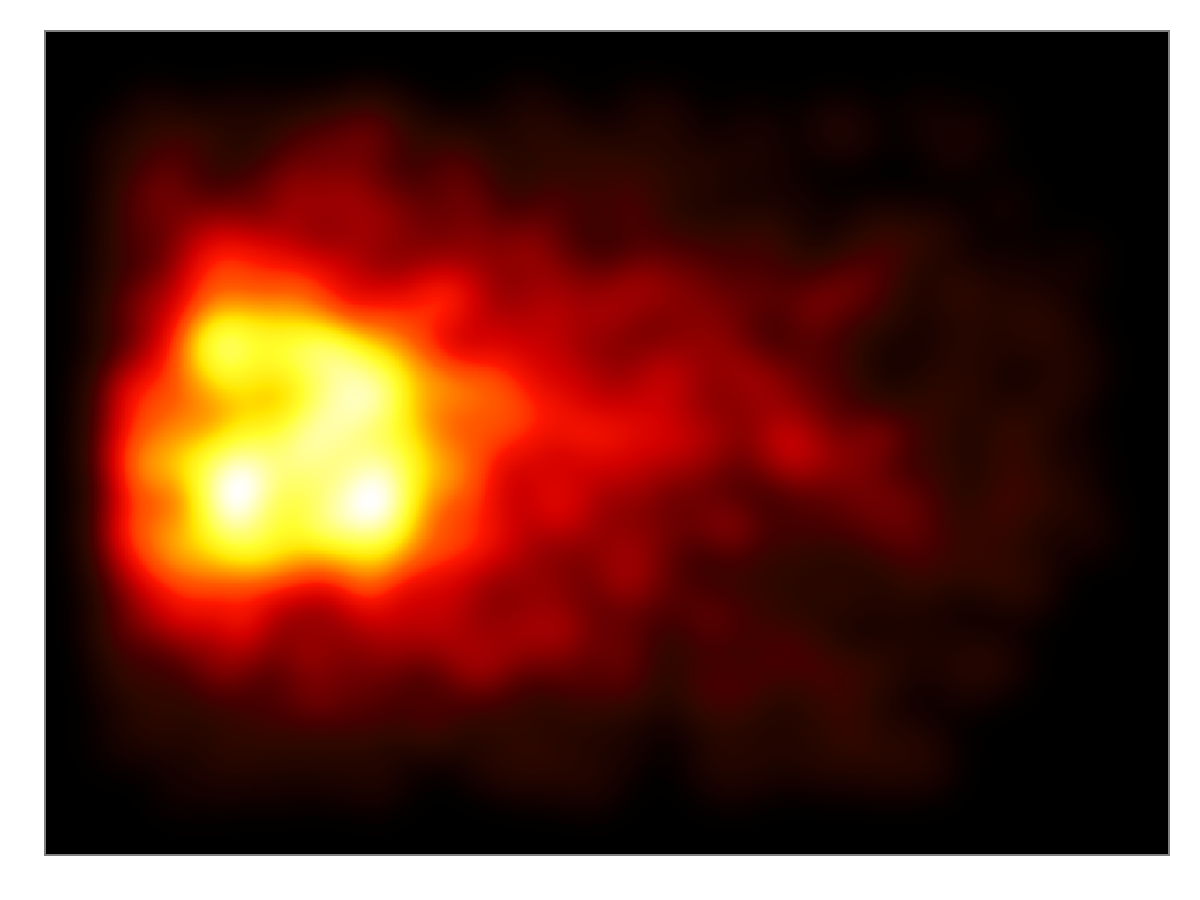
\includegraphics[width=3cm]{../scripts/heatmaps/SaccadicFlowMaps/Figures/BBias_21.pdf}}
\subfigure[]{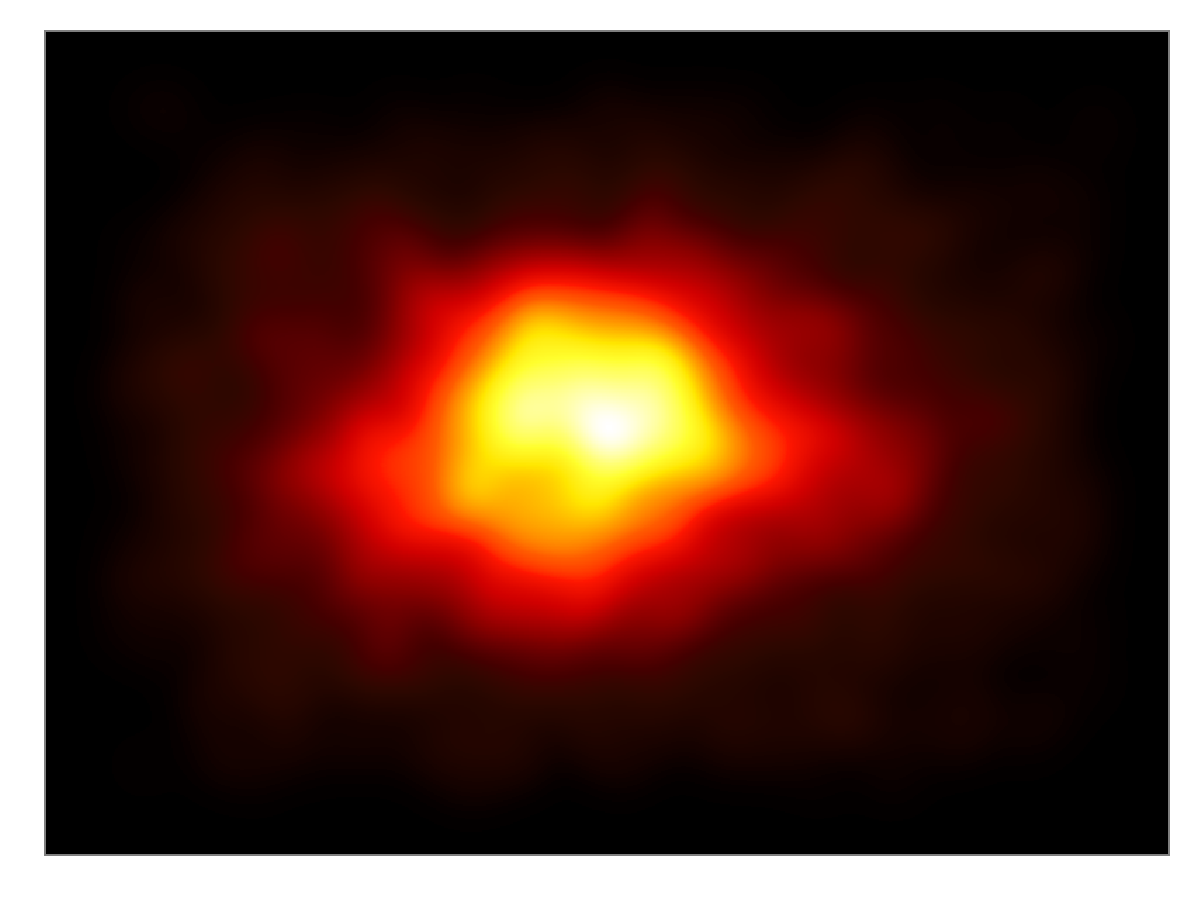
\includegraphics[width=3cm]{../scripts/heatmaps/SaccadicFlowMaps/Figures/BBias_22.pdf}}
\subfigure[]{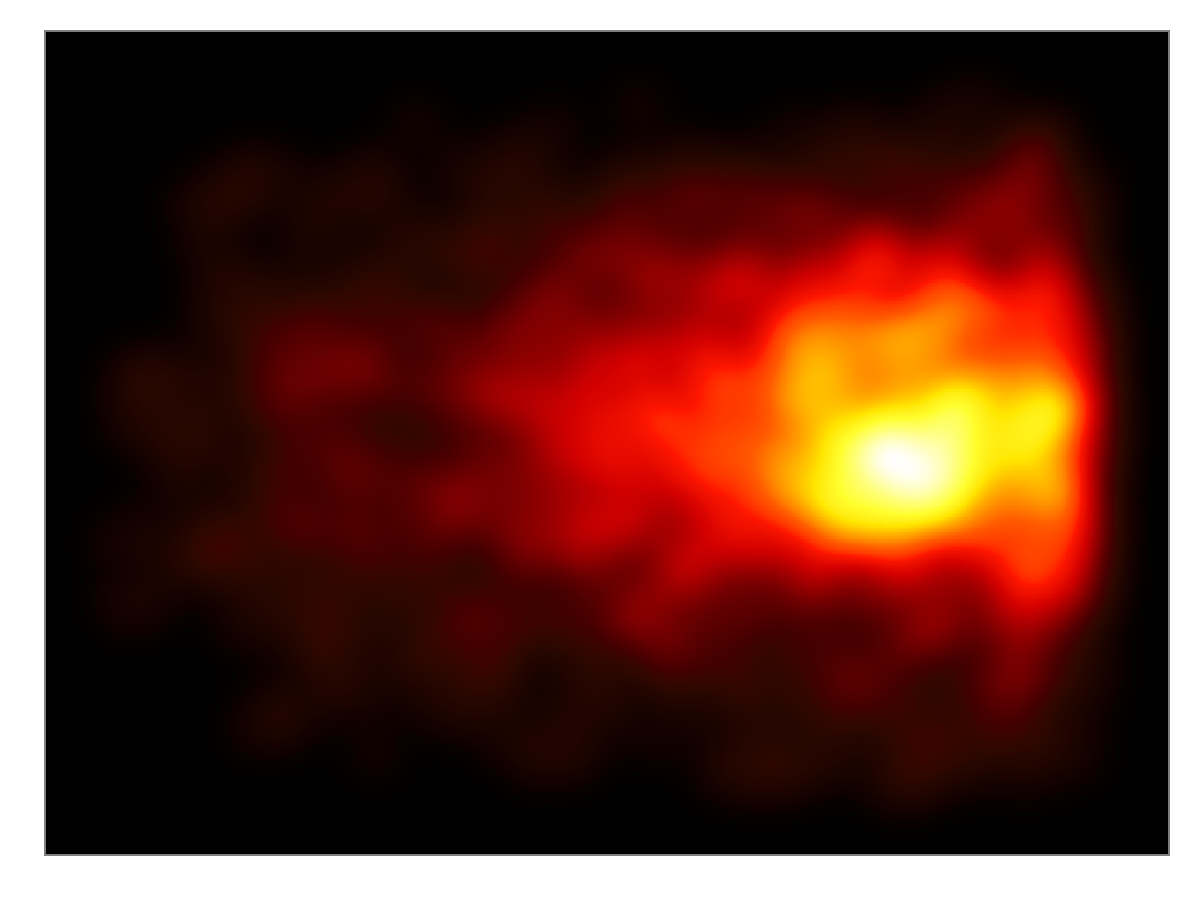
\includegraphics[width=3cm]{../scripts/heatmaps/SaccadicFlowMaps/Figures/BBias_23.pdf}}
\subfigure[]{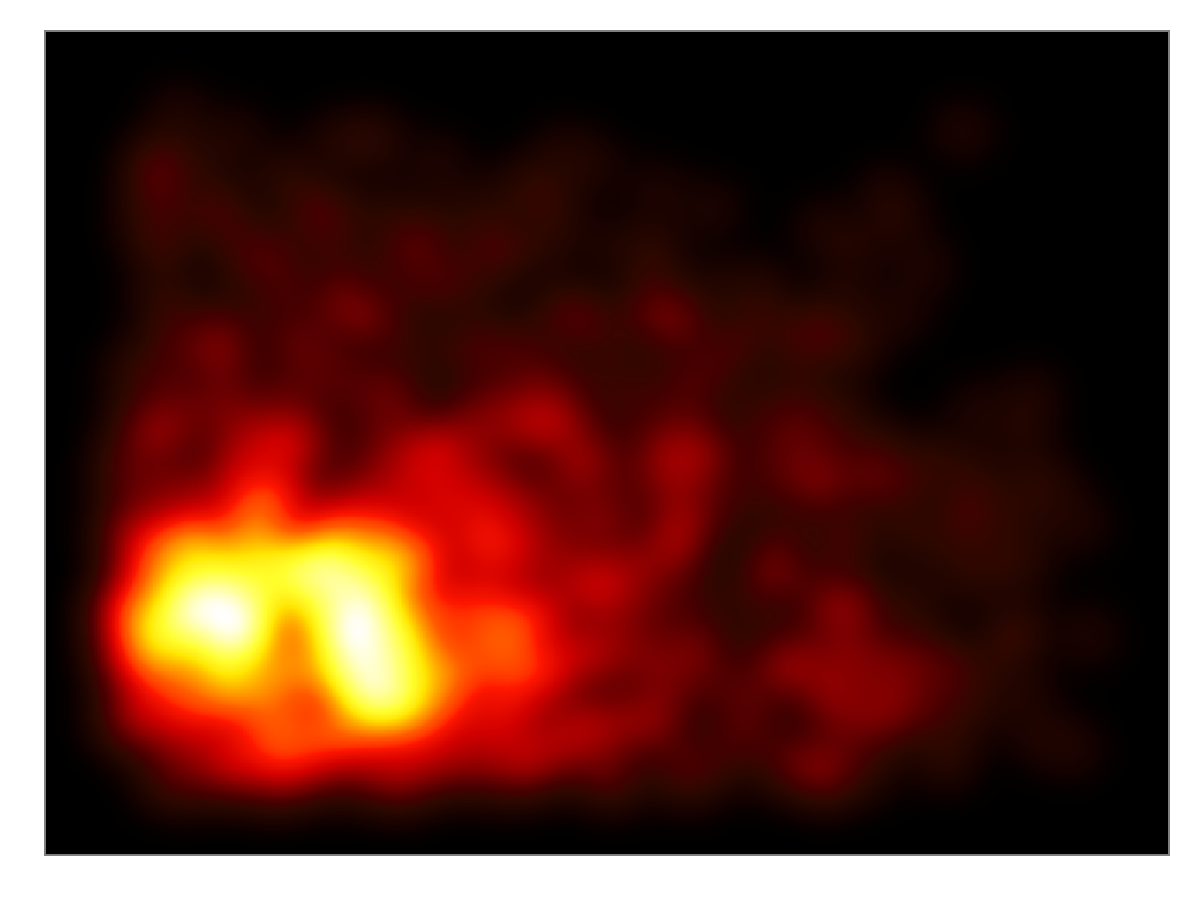
\includegraphics[width=3cm]{../scripts/heatmaps/SaccadicFlowMaps/Figures/BBias_31.pdf}}
\subfigure[]{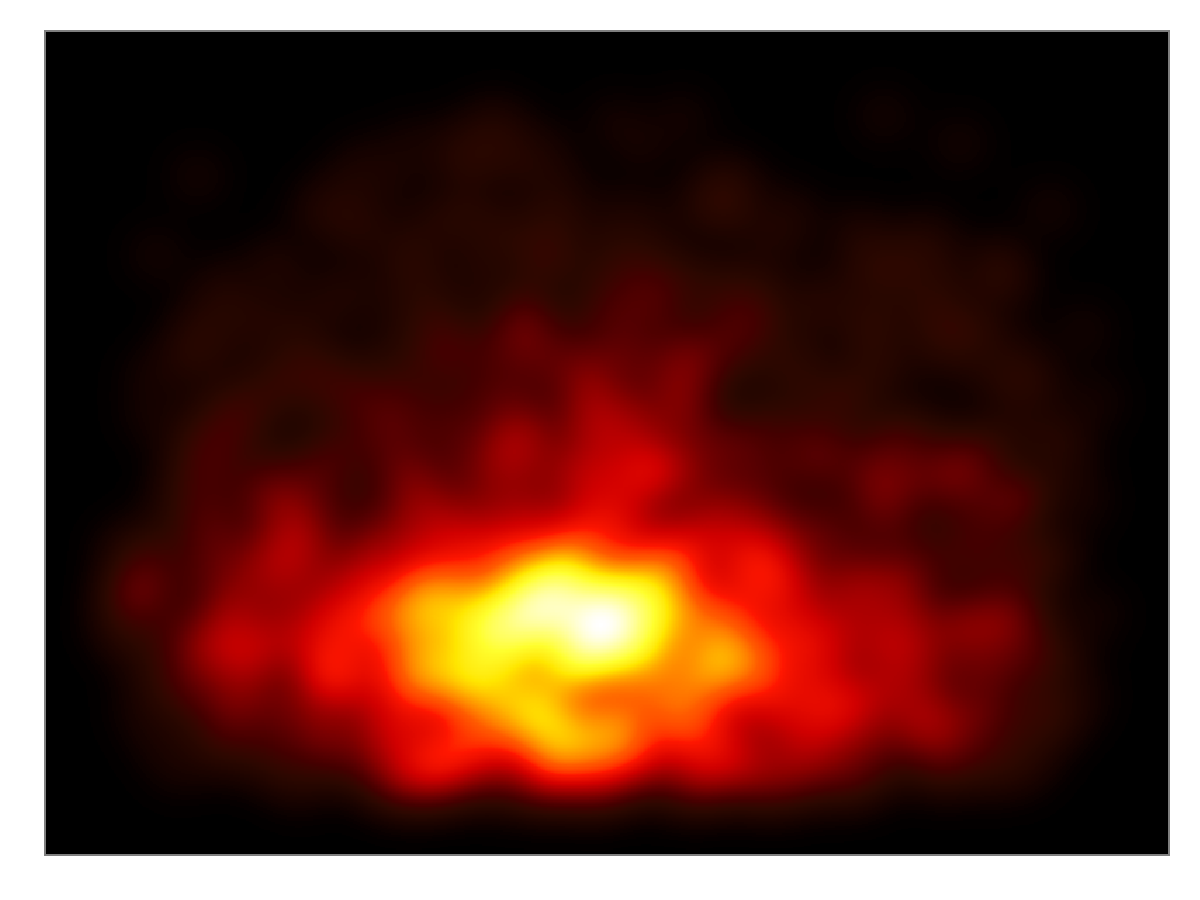
\includegraphics[width=3cm]{../scripts/heatmaps/SaccadicFlowMaps/Figures/BBias_32.pdf}}
\subfigure[]{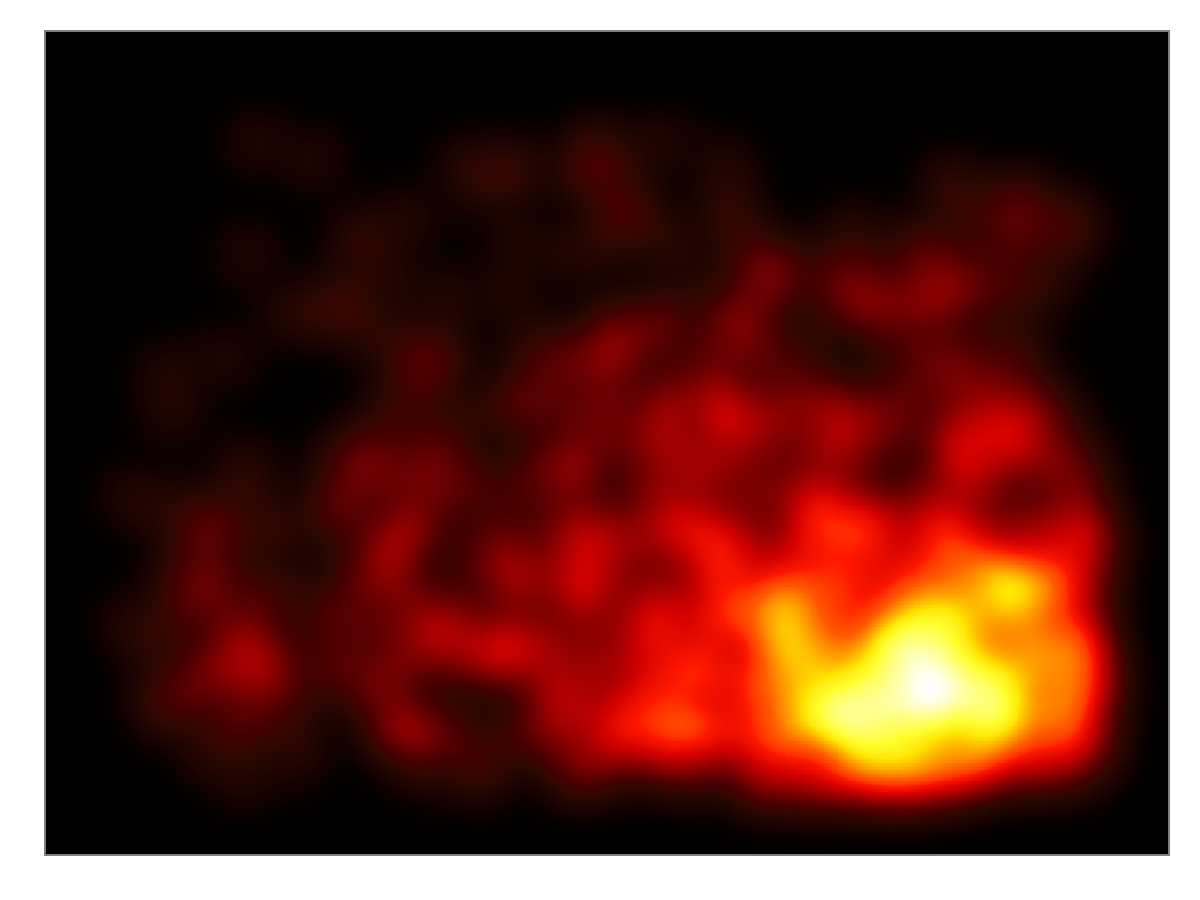
\includegraphics[width=3cm]{../scripts/heatmaps/SaccadicFlowMaps/Figures/BBias_33.pdf}}
\caption{Saccade landing positions from fixations that were in different sections of the screen. Data from each plot has been separated into fixations in 9 spatial bins, with the screen being divided into thirds in both horizontal and vertical aspects.}
\label{fig:empiricalSaccadicFlow}
\end{figure}


%\begin{figure}
%\centering
%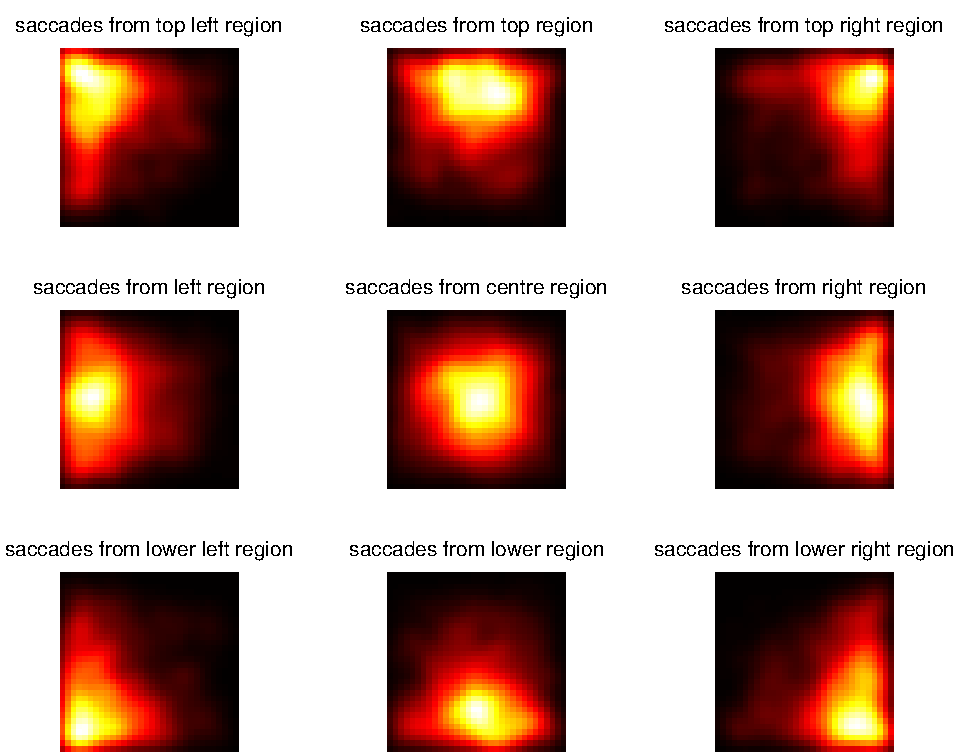
\includegraphics[width=10cm]{figs/saccDistExample.pdf}
%\caption{Empirical example of saccadic flow from \cite{clarke2009}. Fixations come from a visual search %experiment for a target in noise. }
%\label{fig:empiricalSaccadicFlow}
%\end{figure}

\subsection{The present study}
The aim of the present study is to characterise the underlying biases of eye movement with which to understand fixation selection in natural scenes. We extend the previous work by examining [XXstuffXX] and 

%%%%%%%%%%%%%%%%%%%%%%%%%%%%%%%%%%%%%%%%%%%%%%%%%%%%%%%%%%
\section{Methods}
%%%%%%%%%%%%%%%%%%%%%%%%%%%%%%%%%%%%%%%%%%%%%%%%%%%%%%%%%%

\subsection{Datasets}

An overview of the datasets used is given in Tables \ref{tab:datasets} and \ref{tab:setuptable}. Hopefully we can add some more datasets to this. Note, we will note use the \cite{ehinger2009} dataset for training as previous results show that the central bias is due to contextual effects, this dataset behaves slightly differently from the others. However, we will include in in the testing stage. 


\begin{table}
\centering
\small
\begin{tabular}{l|llll}
 & Observers & Images &  Task & Display duration\\
\hline
\cite{clarke2013}     & 24    & 100   & object naming        & 5000 ms\\
\cite{yun2013} - SUN        & 8     & 104   & image description    & 5000 ms\\
\cite{tatler2005}     & 14    & 48     & memory & variable\\
\cite{einhauser2008} & 8    & 93      & object naming & 3000 ms \\
\hline
\cite{tatler2007} - free    & 22    & 120   & free viewing          & 5000 ms\\
\cite{judd2009}         & 15 & 1003      & free viewing & 3000 ms\\
\cite{yun2013} - PASCAL        & 3 & 1000  & free viewing & 3000 ms\\
\hline
\cite{ehinger2009}     & 14 & 912 &  visual search & variable\\
\cite{tatler2007} - search    & 30 & 120 &   visual search & 5000 ms\\
\cite{asher2013}    & 25    & 120      & visual search & variable\\
\end{tabular}

\caption{Summary of the 10 datasets used throughout this study.}
\label{tab:datasets}
\end{table}

\begin{table}
\begin{center}
\small
\begin{tabular}{l|llllll}
 & Eye tracker & \vtop{\hbox{\strut Viewing}\hbox{\strut distance}}
 & \vtop{\hbox{\strut Screen}\hbox{\strut size}}
 & \vtop{\hbox{\strut Image}\hbox{\strut size}}
 & \vtop{\hbox{\strut Viewing}\hbox{\strut angle}}
 & \vtop{\hbox{\strut Chin /}\hbox{\strut head rest}}\\
\hline
\cite{clarke2013} & EyeLink II & 50 cm & 21" & 800 x 600 & 31 x 25\degree & no\\
\cite{yun2013} - SUN & EyeLink 1000 & ? & ? & ? & ? & ?\\
\cite{tatler2005} & EyeLink I & 60 cm & 17" & 800 x 600 & 30 x 22\degree & no\\
\cite{einhauser2008} & EyeLink 1000 & 80 cm & 20" & 1024 x 768 & 29 x 22\degree & yes\\
\hline
\cite{tatler2007} - free & EyeLink II & 60 cm & 21" & 1600 x 1200 & 40 x 30\degree & no\\
\cite{judd2009} & ? & 2 feet & 19" & 1024 x 768* & ? & yes\\
\cite{yun2013} - PASCAL & EyeLink 1000 & ? & ? & ? & ? & ?\\
\hline
\cite{ehinger2009} & ISCAN RK-464 & 75 cm & 21" & 800 x 600 & 23.5 x 17.7\degree & yes\\
\cite{tatler2007} - search & EyeLink II & 60 cm & 21" & 1600 x 1200 & 40 x 30\degree & no\\
\cite{asher2013} & EyeLink 1000 & 55 cm & ? & 1024 x 1280 & 37.6 x 30.5\degree & yes\\
\end{tabular}
\end{center}
\caption{Details of the experimental setups in each of the 10 datasets analysed in the present study. We provide only information reported in the original articles. Question marks indicate information not reported in the original article. *For the Judd et al dataset images varied in pixel dimensions but the majority were at 1024 x 768.}
\label{tab:setuptable}
\end{table}

\subsection{Pre-processing}

As with \cite{clarke-tatler2014} we have normalised all fixations to the image frame, keeping the aspect ratio constant. ie, $(x,y)\in (-1.-1)\times(-a,a)$ with typically $a=0.75$. The initial fixations and saccades were not included in the analysis. Saccades with a start or end point falling outside of the image frame were also removed. 

When fitting saccadic flow models,  we \textit{mirrored} the set of fixations, but adding in reflected copies of the data (reflected in the horizontal, vertical and both midlines). This has two advantages. (i) It is an easy way to make saccadic flow biases in the horizontal or vertical directions. This is similar to how the central bias was defined \cite{clarke-tatler2014}, but by a different mechanism (with the central bias, the model fitting procedure is much simpler and so we just enforced zero mean and 0s in the covariance matrix). (ii) It increases the amount of data available for fitting by a factor of four. This is important as (due to the central bias) there are relatively few saccades that originate from the corners of the images. By equating all corners, we can pool the data and obtain more stable estimates for the underlying distribution. 


\subsection{Training and Testing}

As with \cite{clarke-tatler2014} We will train models on all available data (saccades from all datasets grouped together) and report the resulting model as the baseline we recommended using. In order to check for over fitting, we will additionally evaluate the modelling procedure by training to one single dateset and evaluating over all the others. Our pooled dataset currently consists of over 600,000 saccades over seven datasets. 

When evaluating over the full dataset we will also explore the effect of window-size on the results. The smaller the window, the more accurately we can characterise the behaviour for fixations close to the edge of the image. However, due to the central bias, there are far fewer fixations in these areas and so the distributions fits for these areas are increasingly noisy as the window is moved closer to the edge and with a smaller size. 


\section{Biases}

We will model and discuss saccadic flow, coarse-to-fine, and left v right. 

\subsection{Left v Right}

Initially more fixations to the left half of the image \citep{nuthmann-matthias2014}. We replicate this here (Figure \ref{fig:leftrightDist}).

\begin{figure}
\centering
\subfigure{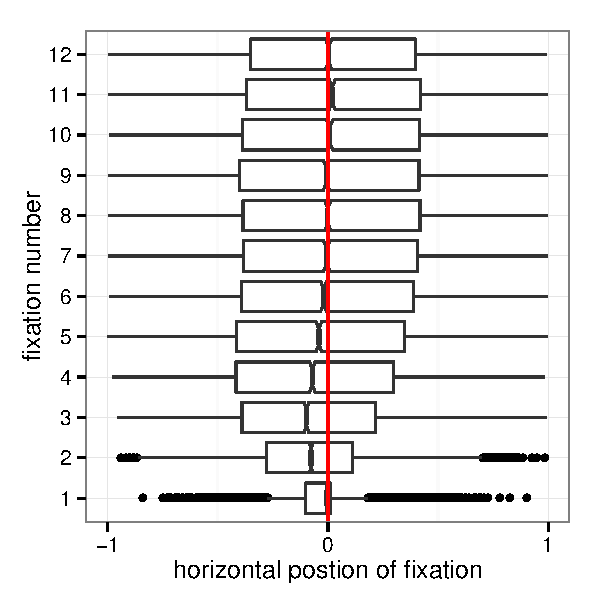
\includegraphics[width=6cm]{../scripts/leftVright/graphs/leftrightbias.pdf}}
\subfigure{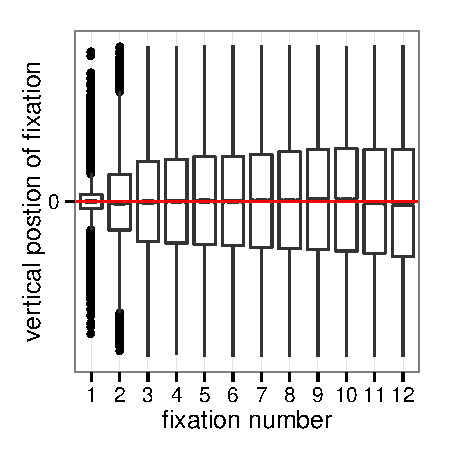
\includegraphics[width=6cm]{../scripts/leftVright/graphs/updownbias.pdf}}
\caption{Distribution of horizontal and vertical fixations by fixation number.}
\label{fig:leftrightDist}
\end{figure}

\subsubsection{Modelling}

However, it has only a very small effect on explaining the varition over whole datasets: Figure \ref{fig:leftrightModelling}.




\begin{figure}
\centering
\subfigure[]{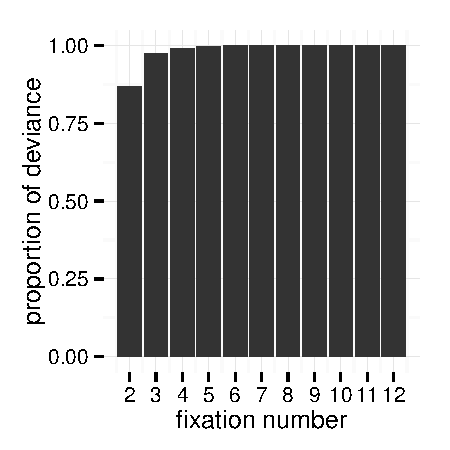
\includegraphics[width=4.1cm]{../scripts/leftVright/graphs/devRatio.pdf}}
\subfigure[]{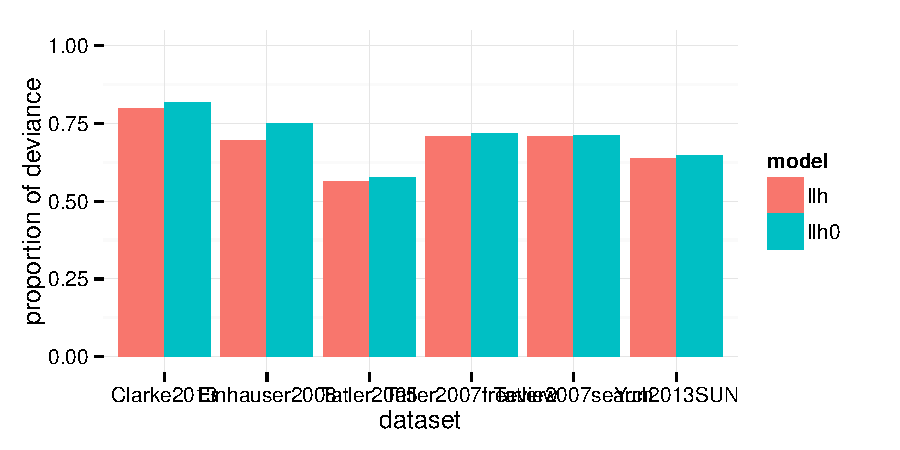
\includegraphics[width=8.2cm]{../scripts/leftVright/graphs/datasetComp.pdf}}
\caption{Modelling results}
\label{fig:leftrightModelling}
\end{figure}

\subsubsection{Discussion}

Hence we will ignore this effect from now on. By treating everything as symmetrical, we lose very little explanitory power, while restricitng the number of parameters, or increasing the amount of data available (by mirroring fixations).

\subsection{Saccadic Flow: Gaussian}

Saccadic flow can be thought of as a generalisation of the central bias. Instead of computing the distribution of all saccadic endpoints in a dataset, we look at the distribution of saccade endpoints given the start points. So for a saccade from $(x_0, y_0)$ to $(x_1, y1)$ we want to model $p(x_1,y_1|x_0, y0)$ This is illustrated in Figure \ref{fig:empiricalSaccadicFlow}.


\subsubsection{Modelling}

To characterise how the distribution of saccadic endpoints varies with the start point, we used a sliding window approach. All saccades that originated in a $n\times n$ window were taken and used to fit a multivariate Gaussian distribution. This window was then moved over the stimuli in steps of $s=0.01$. Parameter sets estimated from windows containing less than 250 datapoints were removed. Multivariate polynomial regression was then used to fit 4-th order polynomials to each of the parameters. We experimented with varying the window size ($n\in\{0.05,0.1, 0.2\}$). However, as this parameter was found to have a negligible result, we only report the results for $n=0.1$.

\begin{figure}
\centering
 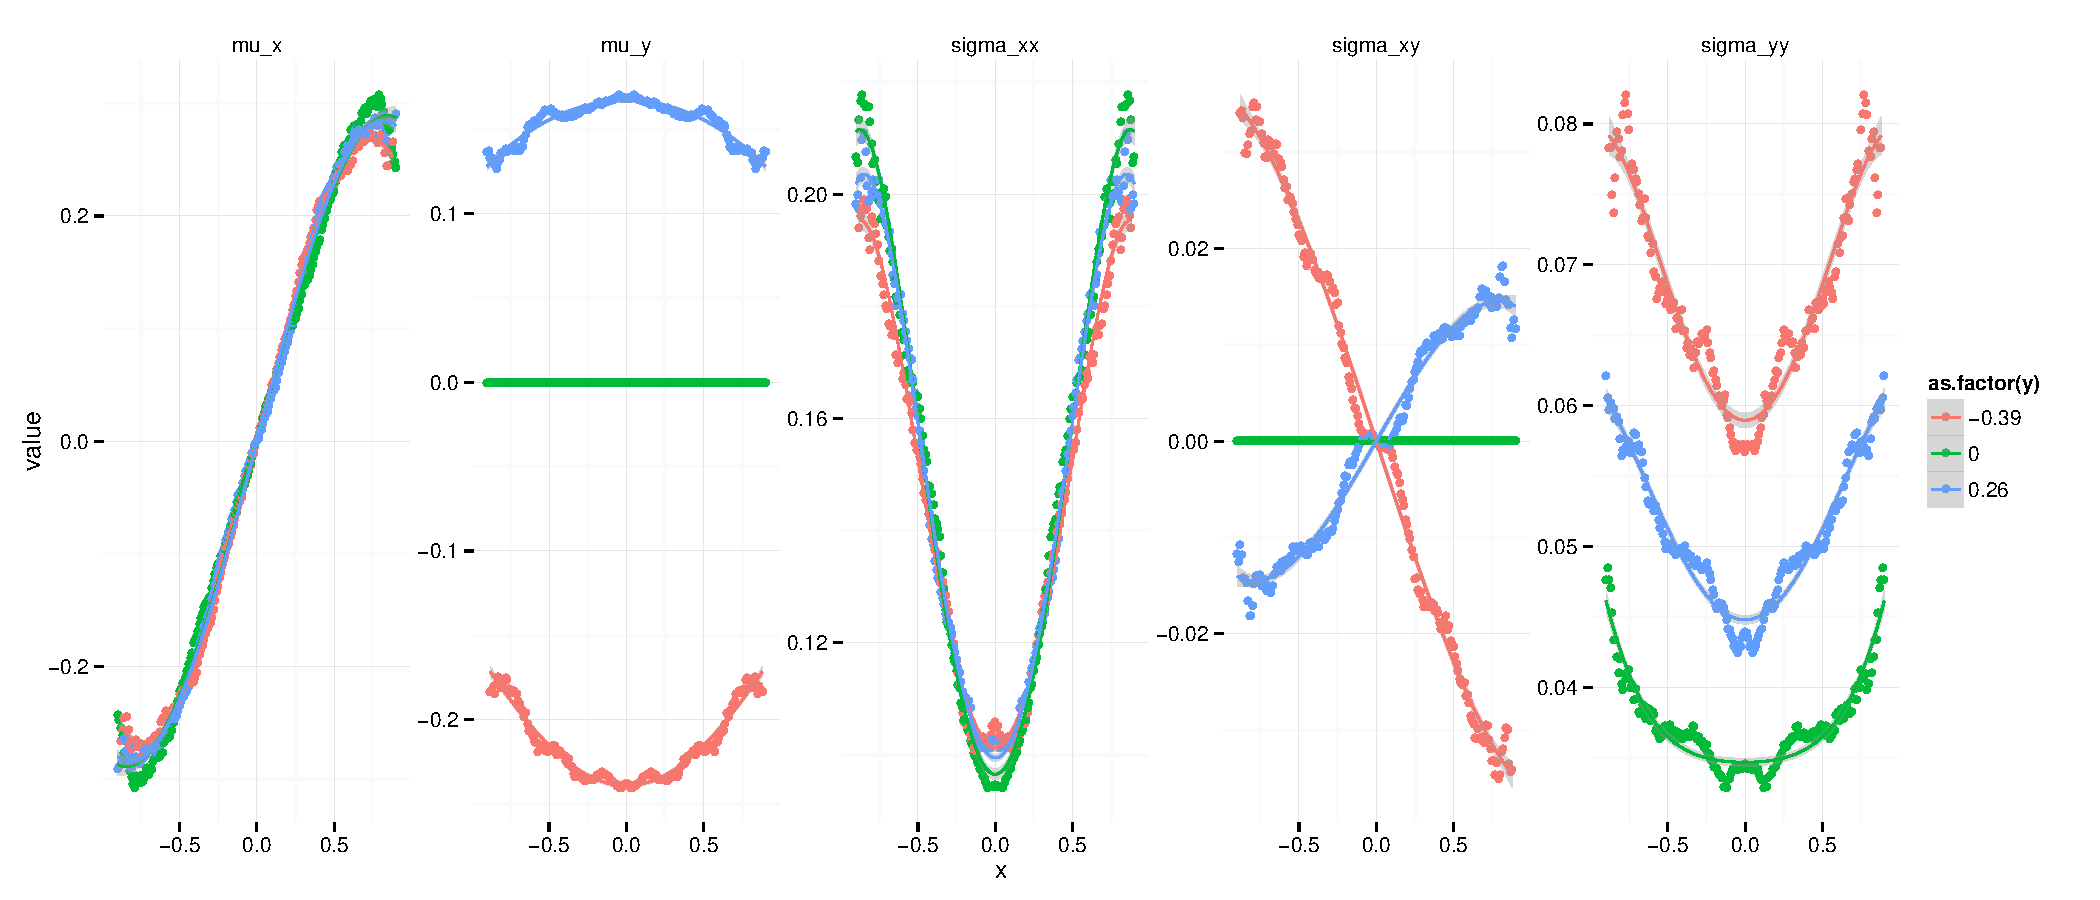
\includegraphics[width=13cm]{../scripts/flow/figs/NparamsChagingOverSpace_ALL.pdf}
\caption{Flow:normal parameters over space. Note this is only a place holder for now. }
\label{fig:nParamsOverSpace}
\end{figure}

\subsubsection{Results}

Figure \ref{fig:nParamsOverSpace} shows how the parameters for the multivariate Gaussian distribution vary over horizontal position for a selection of vertical positions. The regression coefficients given in Table \ref{tab:nParamModel} allow us to estimate the conditional probability of a saccade to $(x_1, y1)$ given the starting fixation $(x_0, y_0)$.



\begin{table}
\centering
\begin{tabular}{c c}
parameter & equation \\
\hline
$\Omega_{x,x}$	& $= 0.33+ 0.38x^2 -0.29y^2 + 0.02x^4 + 0.22y^4$ \\ 
$\Omega_{x,y}$	& $=x + y + x^2 + y^2 + x^3 + y^3 + x^4 + y^4$ \\ 
$\Omega_{y,x}$	& $=x + y + x^2 + y^2 + x^3 + y^3 + x^4 + y^4$ \\ 
$\Omega_{y,y}$	& $=x + y + x^2 + y^2 + x^3 + y^3 + x^4 + y^4$ \\ 
\hline
$\alpha_{x^2}$		& $=x + y + x^2 + y^2 + x^3 + y^3 + x^4 + y^4$ \\ 
$\alpha_{y^2}$		& $=x + y + x^2 + y^2 + x^3 + y^3 + x^4 + y^4$ \\ 
\hline
$\nu$			& $=x + y + x^2 + y^2 + x^3 + y^3 + x^4 + y^4$ \\ 
\end{tabular}
\caption{Parameter model - clearly I still have to fill in all the coefficients!}
\label{tab:nParamModel}
\end{table}

How well does this model account for the fixations in our datasets? Figure \ref{fig:nFlowDevAll} shows the deviance of the flow model expressed as a proportion of the deviance of the Clarke-Tatler central bias. For reference, we also show the results for re-fitting the central bias to each dataset. From this figure, we can see that the flow-normal model approximately halves the deviance. 

\begin{figure}
\centering
 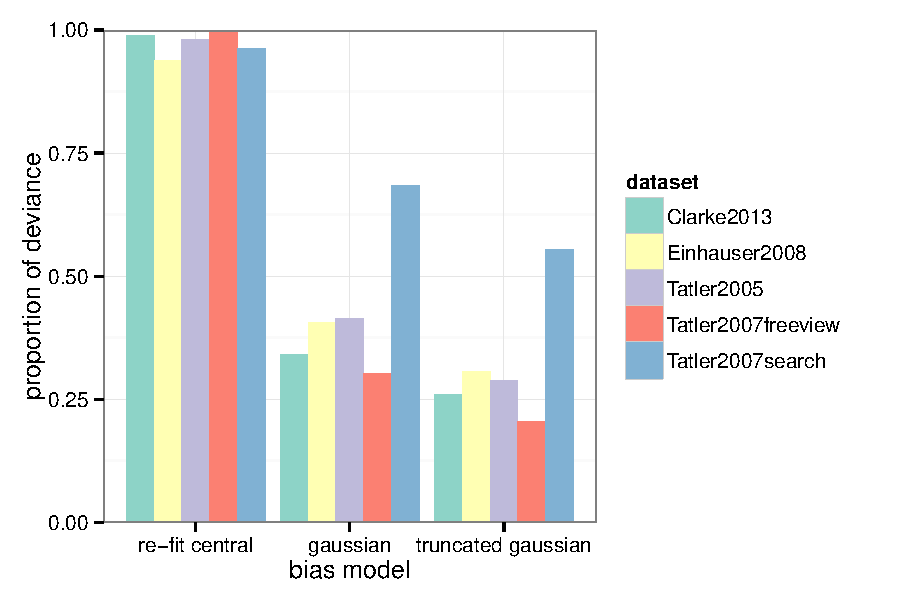
\includegraphics[width=8cm]{../scripts/flow/figs/llh_ALL.pdf}
\caption{Flow:normal deviance results. We can see that re-fitting the central-bias to each specific dataset offers little improvement over using the Clarke-Tatler model, while the flow:normal model decreases the deviance by half.}
\label{fig:nFlowDevAll}
\end{figure}

As the flow:normal model is significantly more complex, requiring nine times as many parameters, it is important to test for robustness. Rather than carrying out $k$-fold cross validation, as we have a large amount of data, we will use a more stringent test, and evaluate how well the flow:normal model trained on just one dataset can explain the variance on the others. These resutls are shown in Figure \ref{fig:nFlowDevCross}.

\begin{figure}
\centering
 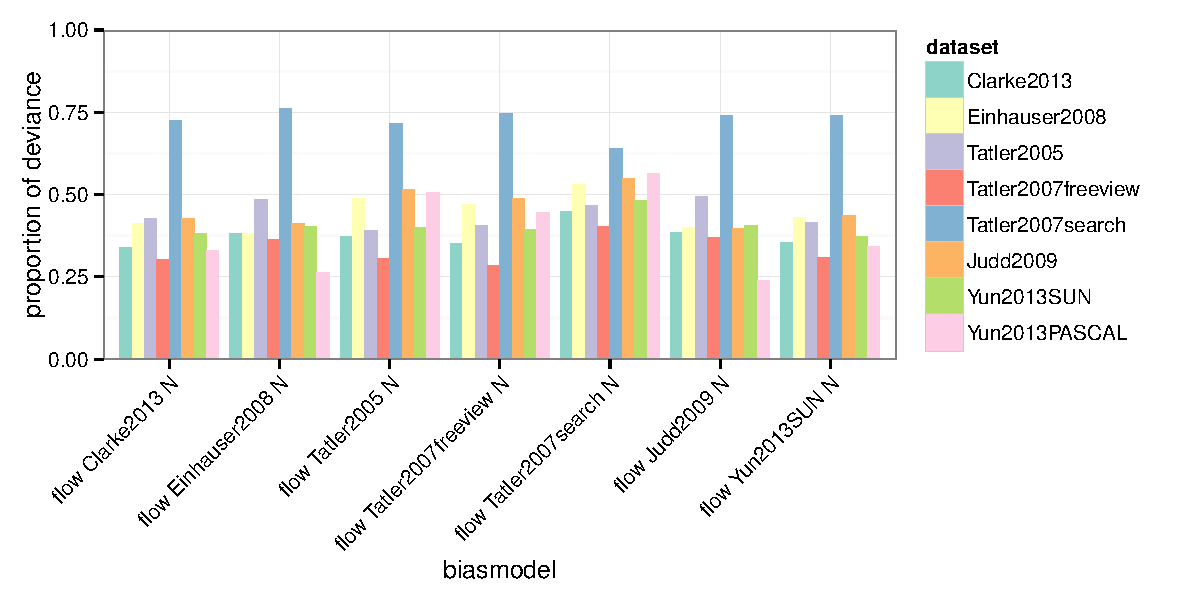
\includegraphics[width=12cm]{../scripts/flow/figs/llh_crossDataset.pdf}
\caption{Flow:normal deviance results over datasets. In general, we can see that bias models trained on different datasets all explain around the same amount of variance in the datasets.}
\label{fig:nFlowDevCross}
\end{figure}

\subsubsection{Discussion}

We put the Flow:normal model forward as a robust prior for image-content independent saccadic behaviour. This model can be thought of as as partner of the Clarke-Tater central bias, and we expect that in some cases, the simpler central bias will be more appropriate, while in others, the more complex flow model is a better choice. We have demonstrated that although this model requires more parameters, it generalises well from one dataset to another and is a far better baseline for modelling a scan-path than the central bias.

There are two main simplifications to our modelling work. First of all, we are using an unbounded distribution (ie, $(x,y)\in \mathbb{R}^2$) to model bounded data. While it is possible to deal with this issue, by either applying a transform $(-1,1)\rightarrow \mathbb{R}$ (such as $z=log(\frac{x'}{1-x'})$, where $x'=\frac{x+1}{2}$), or fitting a truncated multivariate Gaussian, we decided that given the good performance of the model as is, it was not worth adding the additional complexities to our model at this time. 

The second simplification is that we are treating the data as normal. From Figure \ref{fig:empiricalSaccadicFlow} we can see that the data is clearly skewed, particularly in the corners. We will attempt to address these issues in the following section.

\subsection{Saccadic Flow: Skew Normal}
We will model saccadic flow using multivariate skew-$t$ distributions \citep{azzalini2015}. The multivariate skew-normal distribution \citep{azzalini1996} is given by:

\begin{equation}
\phi(z; \lambda) = 2\phi(z)\Phi(\lambda z) 
\end{equation}

for $z \in \mathbb{R}$. I think. 


An example of the the distributions vary with saccadic start point is showing in Figure \ref{fig:exampleSkewNormal}.

\begin{figure}
\centering
\subfigure{\includegraphics[width=3cm]{../scripts/flow/flowFigures/saccEndByX1Y4.pdf}}
\subfigure{\includegraphics[width=3cm]{../scripts/flow/flowFigures/saccEndByX2Y4.pdf}}
\subfigure{\includegraphics[width=3cm]{../scripts/flow/flowFigures/saccEndByX3Y4.pdf}}
\subfigure{\includegraphics[width=3cm]{../scripts/flow/flowFigures/saccEndByX4Y4.pdf}}
\subfigure{\includegraphics[width=3cm]{../scripts/flow/flowFigures/saccEndByX1Y3.pdf}}
\subfigure{\includegraphics[width=3cm]{../scripts/flow/flowFigures/saccEndByX2Y3.pdf}}
\subfigure{\includegraphics[width=3cm]{../scripts/flow/flowFigures/saccEndByX3Y3.pdf}}
\subfigure{\includegraphics[width=3cm]{../scripts/flow/flowFigures/saccEndByX4Y3.pdf}}
\subfigure{\includegraphics[width=3cm]{../scripts/flow/flowFigures/saccEndByX1Y2.pdf}}
\subfigure{\includegraphics[width=3cm]{../scripts/flow/flowFigures/saccEndByX2Y2.pdf}}
\subfigure{\includegraphics[width=3cm]{../scripts/flow/flowFigures/saccEndByX3Y2.pdf}}
\subfigure{\includegraphics[width=3cm]{../scripts/flow/flowFigures/saccEndByX4Y2.pdf}}
\subfigure{\includegraphics[width=3cm]{../scripts/flow/flowFigures/saccEndByX1Y1.pdf}}
\subfigure{\includegraphics[width=3cm]{../scripts/flow/flowFigures/saccEndByX2Y1.pdf}}
\subfigure{\includegraphics[width=3cm]{../scripts/flow/flowFigures/saccEndByX3Y1.pdf}}
\subfigure{\includegraphics[width=3cm]{../scripts/flow/flowFigures/saccEndByX4Y1.pdf}}
\caption{Multivariate skew-$t$ distributions fitted to fixation location, by saccade start point.}
\label{fig:exampleSkewNormal}
\end{figure}

\subsection{Asymmetric flow}

Section to look at what happens if we don't mirror the data.


\section{Using Biases for Better Analysis}

We will use the the central bias \citep{clarke-tatler2014} and \textit{saccadic flow} in some different contexts to see what biases can do for vision research. :p


\subsection{Gaze landscapes}

One technique that is commonly used to visualise the spatial allocation of gaze is to create 'heatmap' plots where colour or luminance are used to indicate the density of fixation on those locations (Figure ~\ref{fig:adjustedHeatmaps}, column 2). Some argue that one problem with visualising data in this way is that they represent all fixations as equal. For example, a fixated location with a fixation of a second would be weighted equally with fixations that lasted half that time. If we want to make an assumption that fixation duration is intimately linked with the importance of that fixation (i.e. we will look longer at more informative information) then we can change our visualisation to weight fixations by their duration (Figure ~\ref{fig:adjustedHeatmaps}, column 3).

One advantage of the \citep{clarke-tatler2014} model, and the saccadic flow model here is that we can represent fixations by the likelihood that they would occur based on the predictions of the models. As there is an image independent tendency to fixate in the centre of the scene (for example), then we might consider that saccades to locations less predicted by these behavioural and oculomotor biases might involve more high-level mechanisms. In Figure ~\ref{fig:adjustedHeatmaps} (column 4 and 5) we present some overlaid heatmap data from the \citep{clarke2013} dataset, where fixations are weighted by the inverse probability of them occuring based on the models of central bias and saccadic flow. These figures reveal that representing data in this manner can allow us to visualise information that was important enough to break the biases of looking at the scene centre, or making saccades in line with our saccadic flow model. We can therefore use this to remove some of the image-independent biases, and reveal the more important image \emph{dependent} information.

\begin{figure}
\includegraphics[width=\textwidth]{figs/adjustedheatmaps.pdf}
\caption{Traditional 'heat map' plots of fixations normalised by the central bias. This method allows us to characterise fixations that are less accountable for by image-independent central biases.}
\label{fig:adjustedHeatmaps}
\end{figure}

Or do we call them hotspot maps?

\subsection{ROC Analysis}

BT to work on this section.
 - by sampling for now. Start with C and T 2014 model then extend to flow model.

Example of using our models rather than shuffle approaches.

\subsection{Flow and Coarse to fine}
To what extent does saccadic flow account for coarse-to-fine dynamics

\subsection{Inverse Yarbus}

Probably drop this section.

Do these biases allow us to improve inverse yarbus performance?

\subsection{Salience}

Does salience explain the less likely saccades? 

Possible follow-up paper?

\section{Discussion}

\cite{}

\subsection{Scenes and natural viewing behaviour}
That observers organise their viewing behaviour on computer screens around the reference frames provided by the bounds of scenes (see also \cite{Stainer:2013ce}) causes problems for relating findings of eye guidance in scenes to eye guidance in natural behaviour, as the bounds of such reference frames are unclear in the real world. While it has been suggested that we tend to fixate near to the centre of our `straight ahead' head position [FOULSHAM WALKING, CRISTINO AND BADDELEY?], there are no discrete edges as are typical in computer based scene viewing paradigms. If fixation locations are constrained by the bounds of the scene, this highlights the care we must take about the generalisations we make from findings in the lab to the real world (see [kingstonepaper 2010]). 






\section*{Acknowledgements}

Thanks to Adelchi Azzalini for advice on using the \texttt{sn} package for \texttt{R}. And mention grants. 

\bibliographystyle{plainnat}
\small
\bibliography{literature}
\end{document}